% This file was created with tikzplotlib v0.10.1.
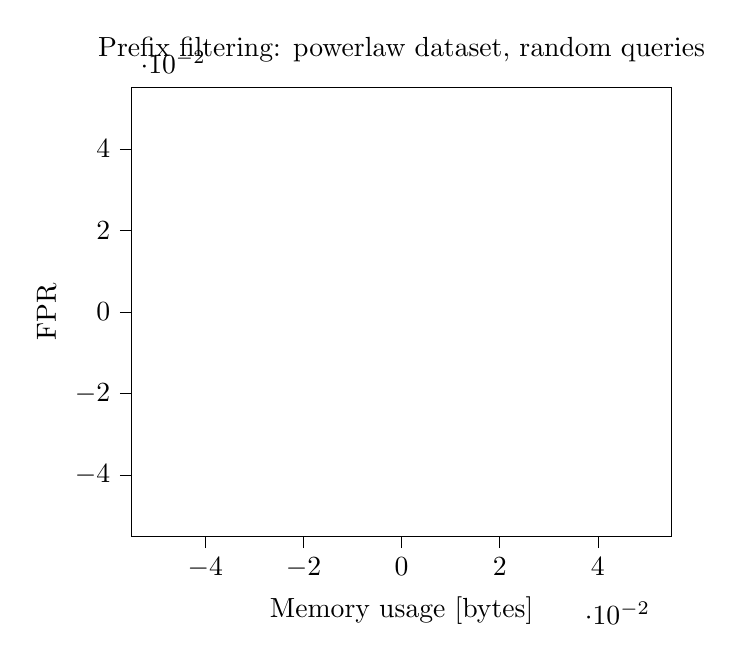
\begin{tikzpicture}

\definecolor{darkgray176}{RGB}{176,176,176}
\definecolor{lightgray204}{RGB}{204,204,204}

\begin{axis}[
legend cell align={left},
legend style={fill opacity=0.8, draw opacity=1, text opacity=1, draw=lightgray204},
tick align=outside,
tick pos=left,
title={Prefix filtering: powerlaw dataset, random queries},
x grid style={darkgray176},
xlabel={Memory usage [bytes]},
xmin=-0.055, xmax=0.055,
xtick style={color=black},
y grid style={darkgray176},
ylabel={FPR},
ymin=-0.055, ymax=0.055,
ytick style={color=black}
]
\end{axis}

\end{tikzpicture}
